% arara: pdflatex
% arara: bibtex
% arara: pdflatex
% arara: pdflatex
\documentclass{llncs}

\usepackage[numbers]{natbib}

\let\oldcite\cite
\let\cite\citep
\let\citeA\oldcite
\let\citeNP\oldcite
\let\citeyear\citeyearpar

\usepackage[table,dvipsnames]{xcolor}

%\usepackage{colortbl}

\usepackage{framed}

\usepackage{tikz}
\usetikzlibrary{calc}
\usetikzlibrary{positioning,backgrounds,fit,arrows,arrows.meta,shapes,shadows}
\usetikzlibrary{shapes.multipart}
\usepackage{pgflibraryarrows}

\usepackage{wrapfig}


\usepackage{latexsym}
\usepackage{amsfonts,amsmath,amssymb}
\usepackage{url}
\usepackage[utf8]{inputenc}
\PassOptionsToPackage{hyphens}{url}
\usepackage{hyperref}
\makeatletter
\g@addto@macro{\UrlBreaks}{\UrlOrds}
\makeatother
%\usepackage[hyphenbreaks]{breakurl}
%\usepackage[hyphens]{url}
\hypersetup{colorlinks=false,pdfborder={0 0 0}}
%\usepackage{textcomp}
%\usepackage{longtable}
\usepackage{multirow,booktabs}

\newcommand{\patternname}[1]{\hyperref[sec:#1]{{\sc #1}}}
\newcommand{\patternnameext}[1]{{\sc #1}}
\newcommand{\patternnameplural}[1]{\hyperref[sec:#1]{{\sc #1s}}}
\newcommand{\patternnameposesssive}[1]{\hyperref[sec:#1]{{\sc #1's}}}

\usepackage{collect}

%% \makeatletter
%% \newcommand{\store}[2]{\definecollection{#1}
%% \begin{collectinmacro}{\@nameuse{#1}}{}{}
%% #2
%% \end{collectinmacro}%
%% \@nameuse{#1}
%% \makeatother

\title{Patterns of Peeragogy}
\author{Joseph Corneli \and
Charles Jeffrey Danoff \and
Charlotte Pierce \and 
Paola Ricaurte \and 
Lisa Snow Macdonald}

\institute{Department of Computing, Goldsmiths College, University of London \\
\url{j.corneli@gold.ac.uk}\\[.5mm]
Mr Danoff's Teaching Laboratory \\
\url{danoff.charles@gmail.com}\\[.5mm]
Pierce Press and Independent Publishers of New England \\
\url{charlotte.pierce@gmail.com}\\[.5mm]
Department of Cultural Studies, Tecnol\'ogico de Monterrey \\
\url{ricaurte.paola@gmail.com}\\[.5mm]
independent researcher and consultant, Los Angeles\\
\url{snowinla@yahoo.com}
}

\begin{document}

\maketitle

\begin{abstract}
We describe nine design patterns that we have developed in our work on the Peeragogy project, in which we aim to help design the future of learning, inside and outside of institutions, drawing on the principles of free/libre/open source software and free culture.  We use these patterns to build an ``emergent roadmap'' for the project.  Our use of design patterns has some novel features that will be relevant to others working in projects with emergent structure.

\keywords{peer production, peer learning, design patterns}
\end{abstract}

%% \begin{itemize}
%% \item[{\bf Week of June 8}] Peeragogy Project and Roadmap, comments \#17--\#27.  JC: I've made an initial revision, changing ``Peeragogy Project'' to ``Peeragogy''.  See text in green below.  Roadmap is orange, meaning ``on deck'' but no major changes have been made there yet.
%% \item[{\bf Week of June 15}] Use or Make and Carrying Capacity, comments up to \#36.  JC: I've made initial revisions, circulated by email.  Lisa has given some thoughtful comments there, some of that has been merged in here but not all. ``Use or Make'' now retitled as ``Reduce, Reuse, Recycle''.
%% \item[{\bf Week of June 22}] A Specific Project and Wrapper.  JC: I've revised ``A Specific Project''.  I'm wondering if some of the other items in our upcoming list are redundant.  Specifically, I think ``Creating a Guide'' could be combined with ``Roadmap'' and ``Scrapbook'' could be combined with ``Pattern Audit Routine''.  This would save us a week of time and perhaps we could use that to get some more feedback.  It would also save some space in the final paper.
%% \item[{\bf Week of June 29}] Heartbeat and Creating a Guide
%% \item[{\bf Week of July 6}] Newcomer and Pattern Audit Routine
%% \item[{\bf Week of July 13}] Scrapbook and Distributed Roadmap
%% \item[{\bf Week of July 20}] Make sure to submit the revised paper
%% \end{itemize}

\section{Introduction}\label{sec:Introduction}

Readers will have encountered \emph{peer production}, at least in applications like Wikipedia, StackExchange, and free/libre/open source software development.   In the Peeragogy project,  we aim to build upon these inspiring examples to help design the future of education.  
We have found design patterns tremendously useful for organizing our thinking about these matters.  However, there is a key difference between our pattern catalog and previous collections of design patterns that touch on similar domains -- like \emph{Liberating Voices: A Pattern Language for Communication Revolution} \cite{schuler2008liberating} and \emph{Pedagogical Patterns: Advice for Educators} \cite{bergin2012pedagogical}.  What makes this project different is that we use our pattern catalog as our primary project management tool.
% -- our way of ``synthesizing form'' \cite{alexander1964notes}.

A convincing implementation of Christopher Alexander’s idea of patterns as a ``living language'' \cite[p.~xvii]{alexander1977pattern} was realized with one of the earliest applications of wiki software developed by Ward Cunningham: the Portland Pattern Repository.  What we have developed is a further iteration of this idea.   Our pattern template is quite traditional: our innovation is to add a ``What's next'' annotation to each pattern, which anticipates the way the pattern will continue to ``resolve'' in the context of our project. 

% The patterns we introduce here focus on negotiating the execution and implementation of solutions in their practical context.
%  This often requires compromise, adjustments and even restarts.  

At a more philosophical level, our approach is all about human interaction, and the challenges, fluidity and lack of predictability that comes with it.  Something that works for one person may not work for another or may not even work for the same person in a slightly different situation.  Nevertheless, it is hard to argue with a formula like ``do X to get Y.'' In our view, other pattern languages often achieve this sort of common sense rationality, and then stop.  Failure in the prescriptive model only begins when people start trying to define things more carefully and make context-specific changes -- when they actually try to put ideas into practice.  The problem has to do with the inevitable distance between ``do as I say'' and ``do with me.''  
%One is put in mind of Alfred Korzybski's famous remark: ``the map is not the territory.''  

Our aim in this paper is to outline a new approach to education drawing on the principles of free/libre/open source software (FLOSS) and open culture.  In order to do this, we attempt to discuss these principles in an actionable, hands-on way.  Mako Hill suggests that one recipe for success in peer production projects is to take a familiar idea -- the canonical example is an encyclopedia -- and make it easy for people to participate in building it \cite{almost-wikipedia}.  Here, our inspiring familiar idea is the university.  This is the \emph{map} (Figure \ref{madison-map}), but the \emph{territory} is the tacitly-familiar idea of peeragogy.  

\begin{wrapfigure}{l}{.52\textwidth}
\vspace{-.2cm}
\begin{center}
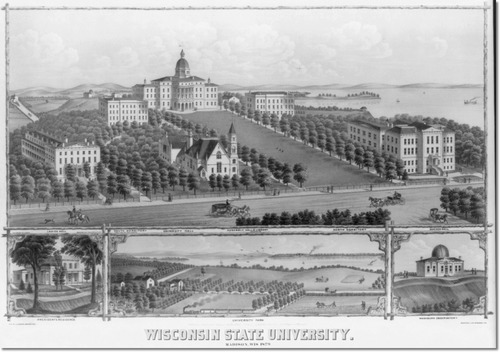
\includegraphics[width=.5\textwidth,trim=0 30 10 2, clip=true]{wisconsin-map}
\end{center}
\vspace{-.1cm}
\caption{A prototypical university.  Caption reads: ``Wisconsin State
  University, Madison, Wis. 1879''.  Inset captions describe the
  pictured buildings: ``Ladies Hall, South Dormitory, University Hall,
  Assembly Halls \& Library, North Dormitory, Science Hall, President's
  Residence, University Farm, and Washburn Observatory.''  Public
  domain.\label{madison-map}}
\vspace{-.3cm}
\end{wrapfigure}

Our model university is not separate from the life of the state or its
citizenry, but aims to ``assume leadership in the application of
knowledge for the direct improvement of the life of the people in
every sphere'' \cite[p. 88]{curti1949university}.  Although we frame
our considerations here in terms of the future of education, peeragogy
is not just for teachers and students, but for anyone with a
commitment to learning.  We use the patterns of peeragogy to
\emph{constitute and occupy practical or speculative problems as such}
\cite[p.~204]{deleuze1994difference}.
%
Our patterns are a living language just insofar as they are linked to
action.  They remain open ended, and in sharing them we invite
critical engagement and argument.

% Till Sch{\"u}mmer \emph{et al.}~have emphasized that pattern authors ``talk about what by definition is tacit'' and highlight the role of nonverbal communication ``needed to communicate the unspeakable'' \cite[p.~9]{schummer2014beyond}.

The essence of peeragogy is to combine an accessible approach with reflective practice.   We seek to develop a richer understanding of collaborative interaction.  This work is relevant to giving the often vague idea of ``openness'' a more concrete meaning, and will have applications within and beyond peer production.  Our approach to emergent organization is likely to be of interest to theorists in fields like organization studies and, perhaps surprisingly, computer science, where researchers are increasingly making use of social approaches to software design and development (e.g., via the \href{http://www.agilemanifesto.org/}{Manifesto for Agile Software Development}) as well as agent-based models of computation and learning \cite{minsky1967programming,poetry-workshop}.

The next section introduces \patternname{Peeragogy} more explicitly in the form of a design pattern.  Sections \ref{sec:Roadmap}--\ref{sec:Scrapbook} present the other patterns in our catalog.  Figure \ref{fig:connections} illustrates their interconnections.  The key forces that apply within the patterns' context are highlighted in bold face.  Each pattern concludes with a short summary and a ``What's next'' annotation.  Section \ref{sec:Distributed_Roadmap} collects these ``next steps'' and summarizes the outlook of the Peeragogy project.  Section \label{sec:Case Studies} includes two short case studies show how the patterns can be applied -- first, in an analysis of current Wikimedia projects, and second to a hypothetical future university.  Section \ref{sec:Conclusion} reviews the contributions made in the paper, positioning this work as a hands-on complement to existing sociological and historical research about peer production (surveyed in \cite{benkler2015peer}).

\begin{figure}
\vspace{-.9in}
{\centering
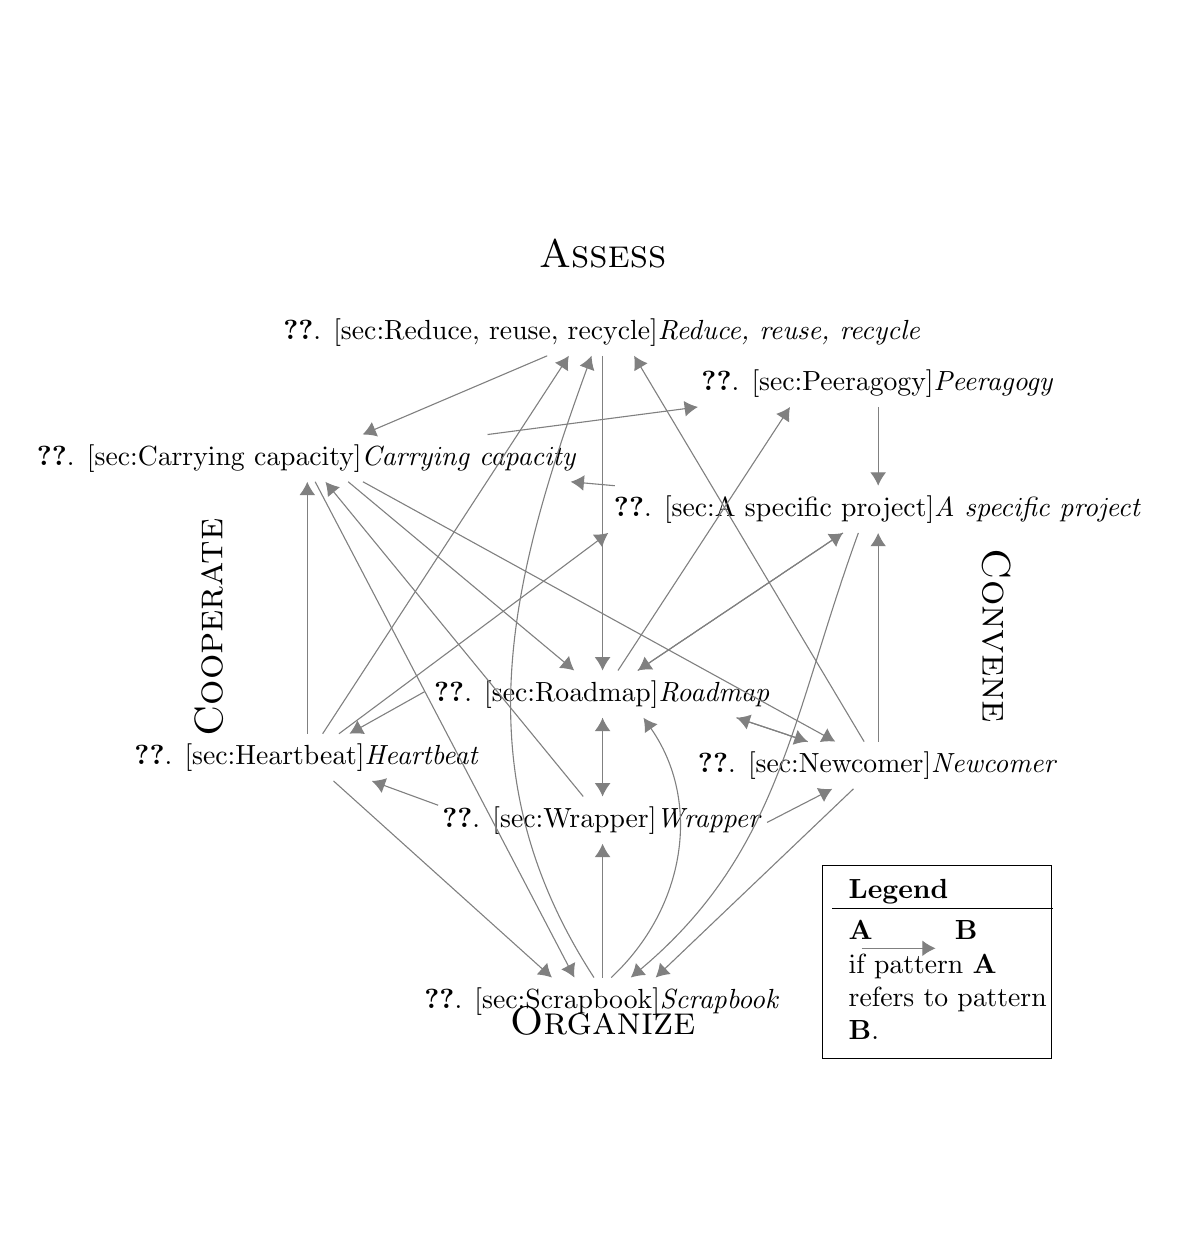
\begin{tikzpicture}[dot/.style={circle,inner sep=1pt,fill,name=#1}]
%\draw[step=1cm,gray,very thin] (0,0) grid (10,10);
\node (assess) at (5, 9.75) {{\Large {\sc Assess}}};
\node (organize) at (5, 0) {{\Large {\sc Organize}}};
\node (cooperate)[text width=2cm,align=center,rotate=270] at (10, 5) {{\Large {\sc Convene}}};
\node (convene)[text width=15cm,align=center,rotate=90] at (0, 5) {{\Large {\sc Cooperate}}};

\node(legend)[draw,rectangle,text width=2.67cm] at (9.25,.75) 
{\begin{tabular}{p{2.7cm}@{\hspace{-1mm}}}
\textbf{Legend}\\ \hline\vspace{-2mm} \textbf{A}\hspace{.41in}\textbf{B}\\
if pattern \textbf{A} refers to pattern \textbf{B}.
  \end{tabular}};
\draw[-{Latex[width=2mm]},draw=gray] ([xshift=5mm,yshift=1.75mm]legend.west) -- ([xshift=-14.8mm,yshift=1.75mm]legend.east);

%%%%%%%%%%%%%%%%%%%%%%%%%%%%%%%%%%%%%%%%%%%%%%%%%%%%%%%%%%%%%%%%%%%%%%%%%%%%%%%%%%%%%%%%%%%%%%%%%%%%%
\node[below = 5cm of assess] (roadmap) {\ref{sec:Roadmap}. \hyperref[sec:Roadmap]{\emph{Roadmap}}};
\node (reduce) at (5, 8.75) {\ref{sec:Reduce, reuse, recycle}. \hyperref[sec:Reduce, reuse, recycle]{\emph{Reduce, reuse, recycle}}};
\node (carryingcapacity) at (1.25, 7.15) {\ref{sec:Carrying capacity}. \hyperref[sec:Carrying capacity]{\emph{Carrying capacity}}};
\node[below = 3.2cm of carryingcapacity] (heartbeat) {\ref{sec:Heartbeat}. \hyperref[sec:Heartbeat]{\emph{Heartbeat}}};
\node (aspecificproject) at (8.5, 6.5) {\ref{sec:A specific project}. \hyperref[sec:A specific project]{\emph{A specific project}}};
\node[below = 1cm of roadmap] (wrapper) {\ref{sec:Wrapper}. \hyperref[sec:Wrapper]{\emph{Wrapper}}};
\node (newcomer) at (8.5, 3.25) {\ref{sec:Newcomer}. \hyperref[sec:Newcomer]{\emph{Newcomer}}};
\node[below = 1.7cm of wrapper] (scrapbook) {\ref{sec:Scrapbook}. \hyperref[sec:Scrapbook]{\emph{Scrapbook}}};
\node[above = 1cm of aspecificproject] (peeragogyproject) {\ref{sec:Peeragogy}. \hyperref[sec:Peeragogy]{\emph{Peeragogy}}};
%%%%%%%%%%%%%%%%%%%%%%%%%%%%%%%%%%%%%%%%%%%%%%%%%%%%%%%%%%%%%%%%%%%%%%%%%%%%%%%%%%%%%%%%%%%%%%%%%%%%%
\draw[-{Latex[width=2mm]},draw=gray] (peeragogyproject) -- (aspecificproject);
% \draw[-{Latex[width=2mm]},draw=gray] (aspecificproject) -- (par);
\draw[-{Latex[width=2mm]},draw=gray] (aspecificproject) -- (roadmap);
\draw[-{Latex[width=2mm]},draw=gray] (aspecificproject.230) to[out=250,in=40] (scrapbook);
\draw[-{Latex[width=2mm]},draw=gray] (aspecificproject) -- (carryingcapacity);
\draw[-{Latex[width=2mm]},draw=gray] (carryingcapacity.337) -- (newcomer);
\draw[-{Latex[width=2mm]},draw=gray] (carryingcapacity.330) -- (roadmap);
\draw[-{Latex[width=2mm]},draw=gray] (carryingcapacity) -- (peeragogyproject);
\draw[-{Latex[width=2mm]},draw=gray] ([xshift=1mm]carryingcapacity.south) -- (scrapbook.140);
% \draw[-{Latex[width=2mm]},draw=gray] ([xshift=2mm]creatingaguide.160) to[out=-215,in=-67] (carryingcapacity);
\draw[-{Latex[width=2mm]},draw=gray] (heartbeat) -- (aspecificproject.185);
\draw[-{Latex[width=2mm]},draw=gray] (heartbeat) -- (carryingcapacity);
\draw[-{Latex[width=2mm]},draw=gray] (heartbeat) -- (scrapbook.155);
\draw[-{Latex[width=2mm]},draw=gray] (heartbeat) -- (reduce.215);
\draw[-{Latex[width=2mm]},draw=gray] (newcomer) -- ([xshift=4mm]reduce.south);
\draw[-{Latex[width=2mm]},draw=gray] (newcomer) -- (aspecificproject);
% \draw[-{Latex[width=2mm]},draw=gray] (newcomer) -- (creatingaguide.north);
\draw[-{Latex[width=2mm]},draw=gray] (newcomer) -- (roadmap.350);
\draw[-{Latex[width=2mm]},draw=gray] (newcomer) -- (scrapbook.24);
% \draw[-{Latex[width=2mm]},draw=gray] (par) -- (scrapbook);
\draw[-{Latex[width=2mm]},draw=gray] (roadmap) -- (peeragogyproject.195);
\draw[-{Latex[width=2mm]},draw=gray] (roadmap.350) -- (newcomer);
\draw[-{Latex[width=2mm]},draw=gray] (roadmap) -- (wrapper);
\draw[-{Latex[width=2mm]},draw=gray] ([yshift=.3mm]roadmap.west) -- (heartbeat);
\draw[-{Latex[width=2mm]},draw=gray] (roadmap) -- (aspecificproject);
% \draw[-{Latex[width=2mm]},draw=gray] (scrapbook) -- (par);
\draw[-{Latex[width=2mm]},draw=gray] (scrapbook) -- (wrapper);
\draw[-{Latex[width=2mm]},draw=gray] (scrapbook.110) to[out=123,in=250] (reduce.245);
\draw[-{Latex[width=2mm]},draw=gray] (scrapbook.70) to[out=43,in=305] (roadmap.330);
% \draw[-{Latex[width=2mm]},draw=gray] ([xshift=2mm,yshift=-.4mm]reduce.south) -- (creatingaguide);
\draw[-{Latex[width=2mm]},draw=gray] (reduce) -- (carryingcapacity);
\draw[-{Latex[width=2mm]},draw=gray] (reduce) -- (roadmap);
\draw[-{Latex[width=2mm]},draw=gray] ([xshift=.7mm]wrapper.175) -- (heartbeat);
\draw[-{Latex[width=2mm]},draw=gray] ([xshift=-.7mm,yshift=-.3mm]wrapper.360) -- (newcomer);
\draw[-{Latex[width=2mm]},draw=gray] (wrapper) -- ([xshift=2.3mm]carryingcapacity.south);
\draw[-{Latex[width=2mm]},draw=gray] (wrapper) -- (roadmap);

\end{tikzpicture}


\par
}
\vspace{-.9in}
\caption{Connections between the patterns of peeragogy.  An arrow points from pattern \textbf{A} to pattern \textbf{B} if the description of pattern \textbf{A} references pattern \textbf{B}. Labels at the borders of the figure correspond to the main sections of the \emph{Peeragogy Handbook}.\label{fig:connections}}
\end{figure}

% deferring a more detailed elaboration of next steps in the educational arena to future work that will build on this basis.
% Technology has come a long way since Alexander suggested ``you will get the most `power' over the language, and make it your own most effectively, if you write the changes in, at the appropriate places in the book'' \cite[p.~xl]{alexander1977pattern}.
% While Christian Kohls insightfully describes patterns as the unique resolution of the dynamical forces acting in a given context \cite{kohls2010structure,kohls2011structure}.
%%% Patterns come to you through mindful awareness ... Charlotte: I think about patterns all the time now, I think about what makes me productive in a team.
% So, while we speak the same language as other developers of design patterns, our orientation is somewhat different, and our understanding of the word `pattern' is nuanced because we aim to take full account of the lifecycle of patterns.  Our work contributes to a recent ``performative'' turn \cite{schummer2014beyond}, which we believe gets at the heart of what design patterns can do.
%  
% In practical terms, we believe the patterns that we introduce here will be useful for students and educators who want their work to have real-world relevance, to activists and policy-makers who want to develop practicable solutions to large-scale problems, and to employees and managers who, like it or not, find themselves working in distributed teams. 
        % \label{sec:Introduction}


\section{Peeragogy}\label{sec:Peeragogy_Project}
% DK: I question whether the Peeragogy Project is a pattern, or an instance of a pattern. We generally think about patterns as something that can be instantiated. But your project seems like a specific case of the concept.

\subsubsection*{Context}  Architectual maverick Christopher Alexander asked the following questions to an audience of computer programmers \cite{alexander1999origins}: 
\begin{quote}
``What is the Chartres of programming? What task is at a high enough level to inspire people writing programs, to reach for the stars?''
\end{quote}
In order for humanity to pull itself up by its bootstraps, on this planet or any other, we need to continue to learn and adapt.  Computers can help accelerate this process.  In particular, collaborative projects like Wikipedia, StackExchange, and Free/Libre/Open Source Software (FLOSS) represent an implicit challenge to the old ``industrial'' organization of work, and the work of education in particular.  In the context of these free, open, post-modern organizations, not only are individual participants learning and growing, but they can contribute to adapting the methods and infrastructure as they go.

\subsubsection*{Problem} What is the real potential of this new way of organizing the human life-world?  Simply creating a free/open piece of software does not mean that other people will get involved: in fact, the majority of free software projects fail to attract users or contributing developers.  Even a wildly successful project like Wikipedia is a work in progress that can be adapted to \emph{\emph{better} empower and engage people around the world, to develop \emph{richer} and more useful educational content, and to deploy it \emph{more creatively}}.\footnote{\url{https://wikimediafoundation.org/wiki/Mission_statement}}  How to go about this is a difficult question, and we don't know the answers in advance.

\subsubsection*{Solution} \emph{Peeragogy} is our word for the process whereby different people involved with different projects can describe material problems, share practical solutions, and constructively critique works-in-progress.   There are many different ways to go about this -- bug reports, mailing lists, writers workshops, and Q\&A forums are all places where peeragogy can happen.  The integration of a wide range of ideas and inputs are supported by, but do not require, internet access.  We have found that the reflection part of the process is particularly well-matched to Christopher Alexander's idea of a \emph{pattern language}, in which commonly occurring  interconnect elements of an optative design are described in terms of a simple template.  Indeed, thought of as a design pattern, \patternname{Peeragogy} can be understood as an up-to-date revision of Alexander's \patternname{Network of Learning} \cite[p. 99]{alexander1977pattern}.  It \emph{decentralizes the process of learning and enriches it through contact with many places and people} -- in interconnected networks that can reach all over the world.   Importantly, while people involved in a peeragogical process may be collaborating on \patternname{A Specific Project}, they don't have to be direct collaborators outside of the learning context or co-located in time or space.  Peeragogy often takes place in mostly-horizontal relationships between people who have different but compatible objectives.  

\subsubsection*{Rationale}
% DK: I have written many, and shepherded many more, and I don’t think this is the case. However, the effort that goes into writing them makes them more intuitive to read :+)
``Patterns'' can be shared in different ways, and finding better ways to express and share them is the important thing (\emph{NB.}~\cite{meszaros1998pattern} describe common patterns involved in the creation of \emph{design patterns} per se).  The main point is that we can navigate the underlying dynamics better when we understand them.  When we're able to share our learning process fluidly with others, this expands the range of perspectives and can produce new insights.  Peeragogy weds Alexander's vision of a programmer's cathedral to Eric Raymond's vision of the corresponding open source bazaar \cite{raymond2001cathedral} -- and opens the doors to non-programmers.
% Our earlier draft: Well-written design patterns is intuitive to read.  The process of finding and writing good design patterns is more involved, but we can be guided by an intuitive sense of what works.
% DK. I am not quite sure what you mean by this: We can use our design pattern catalog to scaffold our work on other parts of the project -- our technical platform, our Handbook, our meetings -- and to connect with others.  

\subsubsection*{Resolution}
%% Our earlier draft: Writing down this pattern defines some of the key terms for \patternname{Newcomers}, and shows how to use the pattern template introduced schematically above.  Together with Figure \ref{fig:connections}, this pattern begins to show how we are affected by using patterns to build emergent structure.
% DK: I think this misses the point of the Resolution. How did Peeragogy resolve the forces that made the problem challenging? Are the participants better off for having used Peeragogy?
Peeragogy helps people in different projects describe and solve real problems.  This can guide action in ways that we wouldn't have seen on our own.

\begin{framed}
\noindent \emph{What's next.} We intend to revise and extend the patterns and methods of peeragogy to make it a workable model for education.
\end{framed}



    
    
    
    
    
    
   % \label{sec:Peeragogy}
%%% Hello!

\section{Roadmap} \label{sec:Roadmap}

% DK: This is a bit self-referential. You have roadmap embedded throughout the description of the pattern. E.g. the context and problem should be able to describe the situation before the solution has been applied, so you should be able to describe them without the solution name in them.

% DK: How is this different from a Backlog? Who “owns” the roadmap? How are changes made to it? How precise is it? Does it have a time dimension to it? You refer to deadlines later on. Does the roadmap include them? (What do deadlines really mean in a project like this anyhow?) Priority?

\subsubsection*{Motivation} This pattern shows how the group can define the scope of their project and make a realistic plan to address it.  This pattern provides the backbone of our pattern language. 


\subsubsection*{Context} \patternname{Peeragogy} has both distributed and centralized aspects. The discussants or contributors who collaborate on a project have different points of view and heterogeneous priorities, but they come together in conversations and joint activities.

\subsubsection*{Forces}~
\parbox[t]{.85\textwidth}{
\textbf{Variety}: people have different goals and interests in mind.\\
\textbf{Clarity}: some may be quite specific, and some rather vague.\\
\textbf{Coherence}: some of these goals will be well-aligned, others less so.
}

\subsubsection*{Problem} In order to collaborate, people need a way to share current, though incomplete, understanding of the space they are working in, and to nurture relationships with one another and the other elements of this space.  At the outset, there may not even be a coherent vision for a project -- but a only loose collection of motivations and sentiments.  Once the project is up and running, people are likely to pull in different directions.   

\subsubsection*{Solution}  Building a guide to the goals, activities, experiments and working methods can help \patternnameplural{Newcomer} and old-timers alike understand how the nature of their relationship with the project.  %% This guide may be a research question or an outline, an organizational mission statement, or a business plan.
It may combine features of a manifesto, a syllabus, and an issue tracker.  It may be a design pattern or a pattern language \cite{kohls2010structure}.  The distinguishing qualities of a project \patternname{Roadmap} are that it should be adaptive to circumstances, and that it should ultimately get us from \emph{here} to \emph{there}.  By this same token, any given version of the roadmap is seen as fallible.  %% Everyone with an interest in the project should have the right to update it, although in practice not everyone will choose to do so.
% * <Charles Danoff> 15:21:53 29 Nov 2015 UTC-0600:
% Should we add the business canvas?
In lieu of widespread participation, the project's \patternname{Wrapper} should attempt to synthesize an accurate roadmap that is informed by participants' behavior, and should help moderate in case of conflict.  Nevertheless, full consensus is not necessary: different goals, with different \emph{heres} and \emph{theres}, can be pursued separately, while maintaining communication.

\subsubsection*{Rationale} 
% DK: This seems more like advice about how to implement the solution than it is an explanation of how the solution addresses the forces from the context/problem [jc: fixed]
In the Peeragogy project our initial roadmap was an outline of the
first draft of the \emph{Peeragogy Handbook}.  Later, it took the form
of a schedule of meetings following a regular
``\patternname{Heartbeat}'' supplemented by a list of upcoming
submission deadlines.  Most recently, it is expressed in the emergent
objectives listed in Section \ref{sec:Distributed_Roadmap} of the
current paper.  We have seen that a list of nice-to-have features created
in a top-down fashion is comparatively unlikely to \emph{go} anywhere.
A backlog of tasks and a realistic plan for accomplishing them are
vastly different things.  An adaptive roadmap is an
antidote to \patternnameext{Tunnel Vision}
\cite[pp. 121--124]{david2001software}. 

\subsubsection*{Resolution}
% DK: This seems like Rationale to me [jc: fixed]
An emergent roadmap is rooted in real problems and justifiable
solutions-in-progress in all their \textbf{variety} and communicates
both resolution and follow-through.  The process of meshing varied
issues with one another requires thought and discussion, and this
encourages \textbf{clarity}.  The test of \textbf{coherence} is that
% * <Charles Danoff> 15:40:10 29 Nov 2015 UTC-0600:
% lisa: getting everyone on the same page + clarity even if what you're doing is not clear
contributed goals and ideas should be actionable.
%
One quality-control test for the roadmap as a whole is that it should
give a \patternnameplural{Newcomer} a reasonable idea of what it would
mean to participate in the project, and help them decide whether,
where, and how to get involved.
% - what happens if you don't have a roadmap?
The ultimate quality-control test is if it worked, i.e., whether the task(s) the roadmap was created to achieve were achieved.  Without a roadmap, we would never know.  If all of the issues that the roadmap outlines are not resolved, the roadmap itself should be revised.  For example, the early outline of the first draft of the Peeragogy Handbook resulted in publication of the first edition of the book.
%% \subsubsection*{Inversion} 
%% The \patternname{Roadmap} is something of a paradox.  We can't dictate
%% the behavior of other participants, and we often can't even guess
%% ourselves what's coming up.  A peeragogical \patternname{Roadmap}
%% should prepare people for the \emph{absence} of clear step-by-step
%% direction, the \emph{presence} of different view points and
%% priorities, and the consequent need to be relatively self-directed.  This pattern
%% isn't particularly suitable for a project that needs to be managed in
%% a top-down fashion, and that can rely on other coordination tools
%% (like contracts) to manage work.

\subsubsection*{Example 1}  The \emph{Help} link present on every Wikipedia page could be seen as a
localized \patternname{Roadmap} for individual user
engagement.\footnote{\url{https://en.wikipedia.org/wiki/Help:Contents}}
%% It tells users what they can do on the site, and gives instructions
%% about how to do it:
%% \begin{quotation}
%% \noindent 
%% I want to \emph{read} or \emph{find} an article \ldots; 
%% I want to \emph{edit} an article \ldots;
%% I want to \emph{report a problem} with an article \ldots;
%% I want to \emph{create a new article} or \emph{upload media} \ldots;
%% I have a \emph{factual question}\ldots
%% ~[Etc.]
%% \end{quotation}
For someone who is prepared to jump in and get to work, there are
around 30 pages listing articles with various kinds of problems, for
example articles tagged with style issues, or ``orphaned'' articles
(i.e., articles with no links from other pages in the
encyclopedia).\footnote{\url{https://en.wikipedia.org/wiki/Category:Wikipedia_article_cleanup}}\textsuperscript{,}\footnote{\url{https://en.wikipedia.org/wiki/Category:Wikipedia_articles_with_style_issues}}\textsuperscript{,}\footnote{\url{https://en.wikipedia.org/wiki/Category:All_orphaned_articles}}
%
%
Wikimedia previously developed
a detailed strategic plan drawing on community input
\cite{wikimedia2011plan}.  In 2015, a two-week 
Community Consultation was carried out and
synthesized, resulting in ``a direction that will guide the decisions for the organization.''\footnote{\url{https://blog.wikimedia.org/2015/02/23/strategy-consultation/}}\textsuperscript{,}\footnote{\url{https://blog.wikimedia.org/2015/08/27/strategy-potential-mobile-multimedia-translation/}}
%
%
 Community-organized WikiProjects often invite outside involvement on \patternname{A
  specific project}.

\begin{wrapfigure}{r}{.48\textwidth}
\vspace{-2.05cm}
\begin{center}
\includegraphics[width=.46\textwidth,trim=140 30 30 30, clip=true]{alabama-big}
\end{center}
\vspace{-.5cm}
\caption{President's Home, University of Alabama.
%Public domain.
\label{presidents-home}}
\vspace{-1.9cm}
\end{wrapfigure}

\subsubsection*{Example 2}
In a future university run in a peer produced manner, a fancy
President's Residence isn't likely be needed.  Leadership would be
carried out in a more collaborative and distributed manner.  It may be
appropriate for project facilitators to meet together at a University
Hall for the primary purpose of working together on the university's
\patternname{Roadmap}.


\smallskip
\bigskip

% \noindent \begin{minipage}{.45\textwidth}
\begin{framed}
\noindent
\emph{What's Next in the Peeragogy Project}
\definecollection{RoadmapWN}
\begin{collectinmacro}{\RoadmapWN}{}{}
If we sense that something needs to change about the project, that is a clue that we might need to record a new pattern, or revise our existing patterns.
\end{collectinmacro}
\RoadmapWN
\end{framed}
%\end{minipage}

\newpage
             % \label{sec:Roadmap}
\section{Reduce, reuse, recycle} \label{sec:Reduce, reuse, recycle}
% DK: I am not sure about the [old] title of this pattern. The bulk of the body of the pattern seems to be about the reuse. Maybe something like “Don’t Make what you can Use” might fit the spirit better. [fixed]

\subsubsection*{Context}
% DK: This seems like an explanation of the title, not a ``context'' in which a problem is observed.
In a peer production context, you are simultaneously ``making stuff'' and building on the work of others. 
\textbf{The ``library'' of resources we can draw on is vast -- but it is useful only if we can make sense of it.}

\subsubsection*{Problem}
People are often very attached to their own projects and priorities and don't have a sense of how their initiatives can benefit from connection and relationship.  Many projects die because the cost of \patternnameext{\href{http://c2.com/cgi/wiki?ReinventingTheWheel}{Reinventing the Wheel}} [c2] is too high.

\subsubsection*{Solution} While it's a great idea to ``steal like an artist'' don't forget to return the favor and make it possible for other people to build on your work too (Figure \ref{fountain}).  In the Peeragogy project, so far we have gotten away with writing very little new software, and have instead used off-the-shelf and hosted solutions suited to the task at hand (including: Drupal, Google+, Google Hangouts, Google Docs, Wordpress, pandoc, XeLaTeX, Authorea, and Github).  We've connected with many different contributors, each with different problems to solve and different ways of moving the project forward.  Early on we agreed to release our \emph{Peeragogy Handbook} under the terms of the Creative Commons Public Domain Dedication (CC0), the legal instrument that grants the greatest possible leeway to downstream users.\footnote{\url{https://creativecommons.org/publicdomain/zero/1.0/}}  This has allowed us and others to repurpose and improve \emph{Handbook} contents in other settings (including the current paper).

\begin{wrapfigure}{l}{.42\textwidth}
\vspace{-0cm}
\begin{center}
\includegraphics[width=.4\textwidth]{figures/Duchamp_Fountaine/Duchamp_Fountaine.jpg}
\end{center}
\caption{A paradigmatic example of found-art. Caption reads: ``Fountain by R. Mutt, Photograph by Alfred Stieglitz, THE EXHIBIT REFUSED BY THE INDEPENDENTS''. Public domain, via the Wikimedia Commons.\label{fountain}}
\vspace{-0cm}
\end{wrapfigure}

\subsubsection*{Rationale} 
Clearly we are not the first people to notice the problems with wheel-reinvention, including ``missing opportunities, repeating common mistakes, and working harder than we need to.''\footnote{\url{https://blog.wikimedia.org/2013/11/19/learning-patterns-new-way-share-important-lessons/}}  As Willow Brugh of Geeks without Bounds and the MIT Media Lab remarked as a guest in one of our hangouts\footnote{\url{https://www.youtube.com/watch?v=NpyQfYVKfBI}}: people often think that they need to build a community, and so fail to recognize that they are already part of a community.   David Kane, this paper's shepherd for PLoP'15, keenly observed that this pattern can be decomposed along the lines of the keywords in its title:  \emph{Reduce} the panoply of interesting interrelated ideas and methods to a functional core (e.g.~writing a book).  \emph{Reuse} whatever resources are relevant to this aim, factoring in ``things I was going to have to do anyway'' from everyone involved.  \emph{Recycle} what you've created in new connections and relationships.  

\subsubsection*{Resolution}  Peeragogy per se is not new, and it's not something we can bottle and sell. It appears in avocational, academic, and industrial contexts.  Furthermore, as much as innovation is celebrated in our culture, there's something to be said for tradition as well.  Reweaving old material into new designs and new material into existing frameworks, we build a deeper understanding.
%
The project's \patternname{Roadmap} develops by making sense of existing resources -- including worries and concerns.

\subsubsection*{Summary}
``You don't have to do everything yourself.''

\begin{framed}
\noindent 
\emph{What's Next.}
We've spun off the pattern catalog from the \emph{Peeragogy Handbook} into this paper, sharing it with a new community and gaining new perspectives.  Let's look for other parts of the handbook we can spin off!
\end{framed}



    
    
         % \label{sec:Reduce, reuse, recycle}
\section{Carrying capacity}\label{sec:Carrying capacity}

\subsubsection*{Motivation} This pattern can help project participants recognise and communicate their stresses to make themselves and the project more resilient.

\subsubsection*{Context}

One of the important maxims from the world of FLOSS is: ``Given enough
eyeballs, all bugs are shallow'' \cite[p.~30]{raymond2001cathedral}.
A partial converse is also true: there's only so much any one person
can do, since we all have limited time and energy.

\subsubsection*{Forces}~
\begin{tabular}[t]{p{.8\textwidth}@{\hspace{.03\textwidth}}c}
\textbf{Antifragility}: each person's potential can only be realised if people take on enough, but not too much. & {\icon \symbol{"002194}} \\
\textbf{Independence}: in a peeragogy context, it is often impossible to delegate work to others. & 
{\icon \symbol{"0021D7}}
\\
\end{tabular}

\subsubsection*{Problem}

How can we help prevent those people who are involved with the project from overpromising or overcommitting, and subsequently crashing and burning?  First, let's be clear that are lots of ways things can go wrong.  Simplistic expectations -- like \emph{assuming that others will do the work for you} \cite{torvalds-interview} -- can undermine your ability to correctly gauge your own strengths, weaknesses, and commitments.  Without careful, critical engagement, you might not even notice when there's a problem.  Where one person has trouble letting go, others may have trouble speaking up.  Pressure builds when communication isn't going well.  
% At the same time, we all seem to have a lot to learn about how to pay attention and make constructive contributions in situations that are always changing.

\subsubsection*{Solution}

Symptoms of burnout are a sign that it's time to revisit the group's \patternname{Roadmap} and your own individual plan.  Are these realistic?  If you have a ``buddy'' they can provide a reality check.   Maybe things are not \emph{that hard} after all -- and maybe they don't need to be done \emph{right now}.  Generalizing from this: the project can promote an open dialog by creating opportunities for people to share their worries and generate an emergent plan for addressing them \cite{seikkula2006dialogical}.  Use the project \patternname{Scrapbook} to make note of obstacles.  For example, if you'd like to pass a baton, you'll need someone there who can take it.  Maybe you can't find that person right away, but you can bring up the concern and get it onto the project's \patternname{Roadmap}.  The situation is always changing, but if we continue to create suitable checkpoints and benchmarks, then we can take steps to take care of an issue that's getting bogged down.    

\subsubsection*{Rationale}

Think of the project as an ecosystem populated by acts of participation.  As we get to know more about ourselves and each other, we know what sorts of things we can expect, and we are able to work together more sustainably \cite{ostrom2010revising}.
%
We can regulate our individual stress levels and improve collective outcomes by discussing concerns openly.

\subsubsection*{Resolution}

Guiding and rebalancing behaviour in a social context can begin with speaking up about a concern.  When we acknowledge our concerns and those of others, we must take into account our own \textbf{boundedness}.  Being aware of the problems and limitations that others face, we have the opportunity to help out, without impinging on others' \textbf{independence}.   This doesn't mean allowing all possible stresses: we work to stay within the realm of \textbf{antifragility} \cite{taleb2012antifragile}, where stress improves the system, rather than degrading them. 
%
As we share concerns and are met with care and practical support, our actions begin to align better with expectations (often as a result of forming more realistic expectations). 

%% \subsubsection*{Inversion}

%% Sharing concerns takes a certain amount of the collective bandwidth too.  There can be times when we need to accept  current limitations, and accept that a certain amount of pain and frustration is part of the process.  Communication can often help address concerns, but

\subsubsection*{Example 1}
Wikipedia aims to emphasize a neutral point of view, but its users are
not neutral.\footnote{\url{https://en.wikipedia.org/wiki/Wikipedia:Neutral_point_of_view}}
Users ``speak up'' about topics that matter to them.\footnote{\url{https://en.wikipedia.org/wiki/Wikipedia:Activist}}
Coverage and participation are not neutral in another less sanguine sense.
More information on Wikipedia deals with Europe than
all of the locations outside of Europe \citep{graham2014uneven}.
As we remarked in the \patternname{Peeragogy} pattern, most of the
actual work is contibuted by a small percentage of users.
%
The technology limits the kinds of things can be said \cite{graham2014uneven}. 
%% ``the structural inability of the platform itself to incorporate fundamental epistemological diversity.''
%
The total number of active editors has been falling since
2007.\footnote{\url{https://strategy.wikimedia.org/wiki/Editor_Trends_Study/Results}}
Some blame outmoded technology and an insider culture
\cite{simonite2013decline}, or point to a stringent editorial
approach that emerged in response to the site's popularity
\cite{halfaker13rise}.  Others highlight the rise of successful competition, often inspired by wiki models, but driven by ``corporate logic'' \cite{kreiss2011limits,morellintroductory}.

\begin{wrapfigure}{r}{.47\textwidth}
\vspace{-.6cm}
\begin{center}
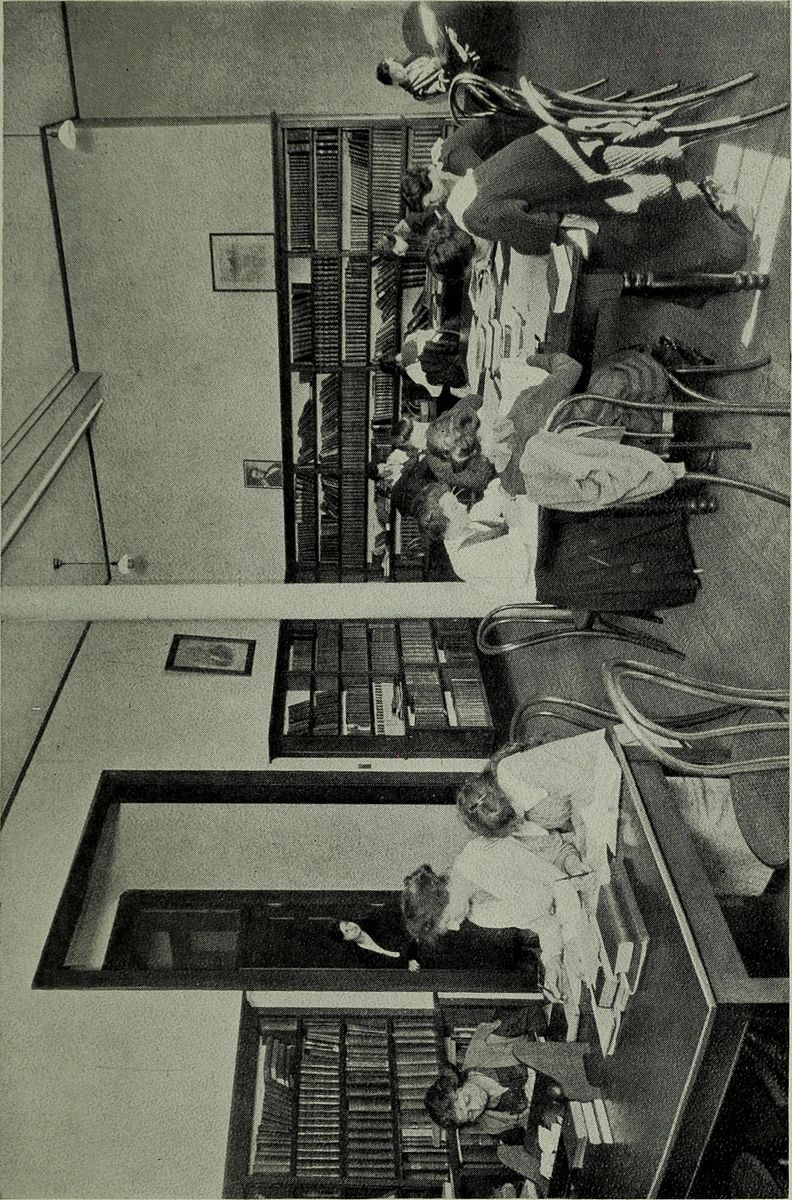
\includegraphics[width=.3\textwidth,angle=-90,trim=0 0 10 10, clip=true]{ladies-hall}
\end{center}
\vspace{-.5cm}
\caption{Queens College, North Carolina.
% Public domain.
\label{ladies-hall}}
\vspace{-.3cm}
\end{wrapfigure}

\subsubsection*{Example 2}
Progressive thinkers have for
some time subscribed to the view that ``there shall be no women in
case there be not men, nor men in case there be not women''
\cite[Chapter 1.LII]{rabelais1894gargantua}.
A separate Ladies Hall seems entirely archaic.
However, in light of the
extreme gender imbalance in free software, and still striking
imbalance at Wikipedia \cite{gender,FM4291}, it will be important to
do whatever it takes to make women and girls welcome, not least
because this is a significant factor in boosting our
\patternname{Carrying capacity}.

%\subsubsection*{Summary}

\begin{framed}
\noindent 
\emph{What's Next in the Peeragogy Project}
\definecollection{CarryingWN}
\begin{collectinmacro}{\CarryingWN}{}{}
Making it easy and fruitful for others to get involved is one of the best ways to redistribute the load.  This often requires skill development among those involved; see \patternname{Newcomer}.
\end{collectinmacro}
\CarryingWN
\end{framed}



  
   % \label{sec:Carrying capacity}
\section{A specific project}\label{sec:A_specific_project}
\subsubsection*{Context}
%DK This seems like a problem…I would think that the context would be something like "there is an existing shared project with a lot of parts/scope, etc."
We often find ourselves confronted with what seems to be a difficult, complex, or even insurmountable problem.  It won't go away, but a workable solution does not present itself either.  Perhaps there is \emph{some} candidate solution, but there are nowhere near enough resources to make it feasible.  

\subsubsection*{Problem}
We are often blinded by our own prejudices and preferences.  Considerable energy goes into pondering, discussing, exploring and feeling stuck.  Meanwhile there may be a strong urge to make more concrete progress, and time is passing by.  In a group setting, when the forward-movers try to act, those who are more wrapped up the experience may attempt to shut them down as they feel that they are being left behind.  However, if moves are being made at random, relative inaction may be the only safe choice.

\subsubsection*{Solution} 
One of the best ways to start to make concrete progress on a hard problem is to ask for help.   Formulating a question helps your thinking become more specific and concrete.  Sometimes you'll see that a solution was within your grasp all along, and you don't actually need to ask the question anymore.  In the case of a really difficult problem, one question won't be enough, but you can repeat the process: turning something that is too large or too ephemeral to tackle directly into a collection of smaller, specific, manageable projects that you can learn something from.  Maintain an overall project \patternname{Roadmap} to keep track of how the smaller pieces relate to the bigger picture.  If you have a fairly specific idea about what you want to do, but you're finding it difficult to get it done, it could be because the project's \patternname{Carrying Capacity} is larger than you thought: you're in a rich landscape, but relatively alone.  Don't just ask for advice in this case: recruit material help.
% DK: This seems a bit speculative, “If you are able…” What steps does this solution entail? How do you know that a project is sufficiently specific? The front part of the pattern makes it sound like the point of view of the pattern is from someone coming into a project looking for something to do, but is there a piece of this pattern for people on a project with ideas about what to do but without the bandwidth to do it? I.e. someone populating the Roadmap with Specific Projects Is there some risk about being too specific about a project?

\subsubsection*{Rationale} 
In our culture, asking for help is often seen as an act of weakness rather than an act of intelligence.
But what we've seen time and again is that asking for help is a recipe for getting specific.
And getting specific is necessary for bringing about change.  Asking for help is one
of the best ways to gain coherence: making yourself understood can go a long way
toward resolving deeper difficulties.  

\subsubsection*{Resolution}
Where you may have felt stuck or realized you were going in circles, getting specific allows forward progress.  The struggle between consensus and action is resolved in a tangible project that combines action with dialog.  Learning something new is a strong sign that this is working.

\begin{framed}
\emph{What's Next.}
We need to build specific, tangible ``what's next'' steps and connect them with concrete action. Use the \patternname{Scrapbook} to organize that process. 
\end{framed}

  % \label{sec:A specific project}
\section{Wrapper}\label{sec:Wrapper}
%OSS: Explain that the wrapper was originally conceived of as a role, is it now? Does it need to be renamed?
\subsubsection*{Motivation} This pattern suggests to find at least one person to fill an important role managing the project's public interface, and keeping participants up to date about activities.

%% \begin{center}
%% \begin{tabular}{l}
%% \textbf{$\leftarrow$\patternname{Roadmap}: If project participants are not all contributing, someone may take charge of the plan.}\\
%% \textbf{$\leftarrow$\patternname{Scrapbook}: Someone may also need to take change of gathering outstanding concerns.}\\
%% \end{tabular}
%% \end{center}

\subsubsection*{Context} You are part of an active, long-running, and possibly quite complex project with more than a handful of participants.  How do you manage?

\subsubsection*{Forces}~
\begin{tabular}[t]{p{.8\textwidth}@{\hspace{.03\textwidth}}c}
\textbf{Interface}: the project shows people how they can use it. & {\icon \symbol{"002136}} \\
\textbf{Familiarity}: the leader/follower dichotomy is easy to understand. &  {\icon \symbol{"0021B2}} \\
\textbf{Equity}: peeragogy aims for fairness. &  {\icon \symbol{"0021BD}} \\
\end{tabular}

\subsubsection*{Problem} In an active project, it can be effectively impossible to stay up to date with all of the details.  Not everyone will be able to attend every meeting (see \patternname{Heartbeat}) or read every email.  Project participants can easily get lost and drift away.  The experience can be much more difficult for \patternnameplural{Newcomer}: joining an existing project can feel like trying to climb aboard a rapidly moving vehicle.  If you've taken time off, you may feel like things have moved on so far that you cannot catch up.  Information overload is not the only concern: there is also a problem with missing information.  If they aren't shared, key skills can quickly become bottlenecks (see \patternname{Carrying capacity}).

\subsubsection*{Solution}
% DK: Be more direct.  Don’t say what “can” be done…just say what to do. [also, typo -jc]
Someone involved with the project should regularly create a wrap-up
summary, distinct from other project communications, that makes
current activities comprehensible to people who may not have been
following all of the details.  In addition, project members should
keep other informative resources like the landing page,
\patternname{Roadmap}, and documentation up to date.  Ensure that
these resources accurately represent the facts on the ground, and
check empirically to see if they really show interested parties how
they can get involved (e.g., the ``dashboard'' pictured in Figure
\ref{dashboard} would have to be kept up to date).  The
\patternname{Wrapper} is both a role, and, sometimes, an artifact.
Our \emph{Handbook}'s cover literally wraps up its contents; the
collaboratively written chat notes from our weekly Hangouts give a
collaboratively-written overview of what was discussed in the meeting.
Meetings themselves can be structured to give people a chance to sum
up what they've accomplished during the week, as well as any problems
they are running into.  Between meetings, each participant is advised
to maintain some sort of ``learning log'' in the form of a personal
\patternname{Scrapbook}, so that outstanding concerns are surfaced and
available to discuss.

\subsubsection*{Rationale}
According to the theory proposed by Yochai Benkler, for free/open ``commons-based'' projects to work, it is important for participants to be able to contribute small pieces, and for the project to have a way to stitch those pieces together \cite{coases-penguin}. The \patternname{Wrapper} helps perform this integrative stitching function. If you value participation, you may have to do some serious work to facilitate access to process.

\subsubsection*{Resolution} 
% DK: This sounds like Rationale
Well-maintained records chronicle the project's history; up-to-date documentation makes the project more robust; a coherent look-and-feel offers an accessible \textbf{interface} to the outside world. Regularly circulated summaries can help to engage or re-engage members of a project, and can give an emotional boost to peeragogues who see their contributions and concerns mentioned, giving less engaged participants the \textbf{familiar} experience of ``following'' someone else's updates. People will judge from experience whether the project strives for \textbf{equity} or strives to maintain hidden power differentials.  

\subsubsection*{Example 1} 
There are many data streams around the Wikimedia project.  They comprise an elaborate \patternname{Wrapper} function for the project, with components that range from Today's Featured Article, which appears on the front page of Wikipedia, to formal annual reports from the nonprofit.\footnote{\url{https://en.wikipedia.org/wiki/Wikipedia:Today\%27s_featured_article}}\textsuperscript{,}\footnote{\url{https://wikimediafoundation.org/wiki/Annual_Report}}

%% That said, citing Wikipedia in academic writing remains controversial.
%% One team of researchers found that, all else equal, when a scientific article is
%% cited on Wikipedia, that does not make it more likely to be cited
%% elsewhere \cite{marashi2013impact}.  These facts suggest that Wikipedia 
%% provides a relatively ``thin'' and non-distorting window on the world.

\subsubsection*{Example 2} In-person meetings are just as relevant for contemporary humans as they were a century ago, even though we often work remotely, and have learned more about how to assemble on the fly \cite{rheingold2007smart}.  Getting together for conventions, dance parties, and commencement ceremonies could comprise an important part of the future university's \patternname{Wrapper} function, even if these events do not always take place in one specific Assembly Hall.

%\subsubsection*{Summary}

\begin{figure}[t]
{\centering
\resizebox{.85\textwidth}{!}{
\begin{tikzpicture}[every node/.style={anchor=south west,inner sep=0pt},x=1mm, y=1mm,]
     \node (fig1) at (0,0)
       {\includegraphics[width=\textwidth,trim=0mm 135mm 0mm 0mm,clip=true]{figures/peeragogy_dashboard_draft1/peeragogy_dashboard_draft1.jpg}};
     \node (fig2) at (55, 15)
       {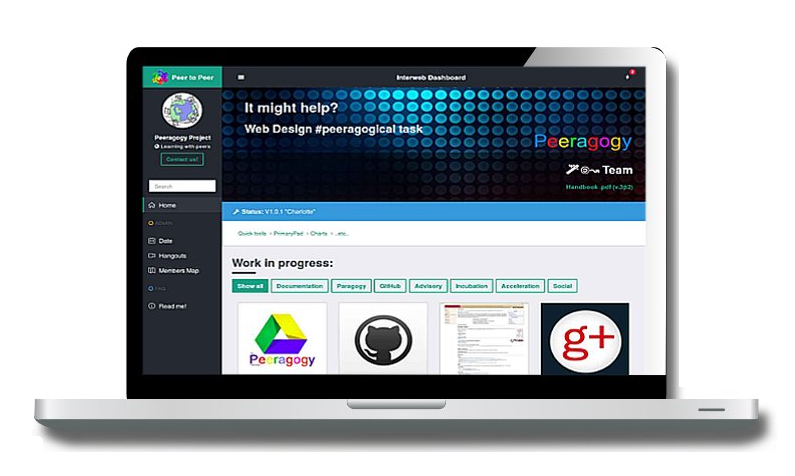
\includegraphics[width=.45\textwidth,trim=10mm 10mm 10mm 10mm,clip=true]{figures/dashboard/dash-trans.png}};  
\end{tikzpicture}
}

\par}
\caption{Design for a Peeragogy project dashboard (sketch by Amanda Lyons, prototype by Fabrizio Terzi; images used with permission).\label{dashboard}}
\end{figure}

\FloatBarrier

\begin{framed}
\noindent 
\emph{What's Next in the Peeragogy Project}
\definecollection{WrapperWN}
\begin{collectinmacro}{\WrapperWN}{}{}
Let's make sure we have protocols in place that enable us to share
progress, and to revise our ``next steps'' if people are getting
stuck.  Let's improve the interaction design for peeragogy.org so that
it's clear how people can get involved.
\end{collectinmacro}
\WrapperWN
\end{framed}    

%\newpage
             % \label{sec:Wrapper}
% DK: My book is out of print now, but the chapter in Rhythm is available online, http://www.informit.com/articles/article.aspx?p=28785 You might find some ideas that lineup with this pattern there
\section{Heartbeat}\label{sec:Heartbeat}

\subsubsection*{Motivation} This pattern can help project participants stay in touch, and stay motivated.

\subsubsection*{Context}
% DK: I think you might be missing some pieces of context….people are busy, the FLOSS project is probably not their day job, etc…
A number of people have a shared interest, and have connected with each other about it.  However, they are not going to spend 24 hours a day, 7 days a week working together, either because they are busy with other things, or because working separately on some tasks is vastly more efficient.

\subsubsection*{Forces}
\parbox[t]{.85\textwidth}{
\textbf{Differentiation}: the time we spend together isn't all equally meaningful.\\
\textbf{Entropy}: something needs to hold the project together, or it will fall apart.
}

\subsubsection*{Problem} How will the effort be sustained and coordinated sufficiently?  How do we know this an active collaboration, and not just a bunch of people milling about?  Is there a \emph{there, there?}  

\subsubsection*{Solution} People seem to naturally gravitate to something with a pulse.  \emph{Once a day} (standups), \emph{once a week} (meetings), or \emph{once a year} (conferences, festivals) are common variants.  When the project is populated by more than just a few people, it's likely that there will be several \patternnameplural{Heartbeat}, building a sophisticated polyrhythm.  A well-running project will feel ``like an improvisational jazz ensemble'' \cite{david2001software}.  Much as the band director may gesture to specific players to invite them to solo or sync up, a project facilitator may craft individual emails to ask someone to lead an activity or invite them to re-engage.  Two common rhythm components are weekly synchronous meetings with an open agenda, combined with \emph{ad hoc} meetings for focused work on \patternname{A specific project}.  The precise details will depend on the degree of integration required by the group.

\subsubsection*{Rationale}  The project's heartbeat is what sustains it. Just as \emph{people matter more than code} \cite{torvalds-interview}, so does the life of the working group matter more than mechanics of the work structure.  Indeed, there is an quick way to do a reality check and find the project's strongest pulse: the activities that sustain a healthy project should sustain us, too (cf. \patternname{Carrying capacity}).
% DK: Help the reader understand what this difference is...

\subsubsection*{Resolution} Noticing when a new \patternname{Heartbeat} is beginning to emerge is a way to be aware of the shifting priorities in the group, and contributes to further \textbf{differentiation}.  This may ultimately be a good source of new patterns. On the other hand, if a specific activity is no longer sustaining the project, stop doing it, much as you would move an out-of-date pattern to the \patternname{Scrapbook} in order to make room for other concerns. The power of the \patternname{Heartbeat} is that the project can be as focused and intensive as it needs to be, working against \textbf{entropy} in the ways that start to be required as time goes by.

\subsubsection*{Example 1} The yearly in-person gathering, Wikimania, is the most visible
example of a \patternname{Heartbeat} for the Wikimedia movement.\footnote{\url{https://meta.wikimedia.org/wiki/Wikimania}}
Local chapters and projects may run additional in-person get-togethers.\footnote{\url{http://wikiconferenceusa.org/}}
Also of note is the twice-yearly call for proposals for individual
engagement grants.\footnote{\url{https://meta.wikimedia.org/wiki/Grants:IEG}}

\subsubsection*{Example 2} Although it may sound quaint, working farms could help to physically
sustain peeragogues, while putting the project's \patternname{Heartbeat} in tune with that of the seasons.  In the
current distributed mode, we tend our windowboxes and allotment gardens.

\begin{framed}
\noindent 
\emph{What's Next.}
\definecollection{HeartbeatWN}
\begin{collectinmacro}{\HeartbeatWN}{}{}
Identifying and fostering new \patternnameplural{Heartbeat} and new working groups is a task that can help make the community more robust.  This is the time dimension of spin off projects described in \patternname{Reduce, reuse, recycle}.
\end{collectinmacro}
\HeartbeatWN
\end{framed}


           % \label{sec:Heartbeat}


% DK: I am not sure that this is a Pattern. It is a role for sure, but is it a solution to a problem? Maybe the name of the pattern is wrong. Something like Welcome Wagon? Something that evokes the response to the Newcomer.
\section{Newcomer}\label{sec:Newcomer}

\subsubsection*{Context}
% DK: This is an interesting point. I am not sure it is Context. Maybe Rationale?
Education assumes we are speaking to a new generation. 
In learning more broadly, the ``audience'' is typically new to the topic, or to some aspect of the topic, that they are learning about.
\textbf{In working to make our project as useful as possible, it seems that there's always something for us to learn, too.}

\subsubsection*{Problem} Newcomers can feel overwhelmed by the amount of things to learn.  They
don't know where to start.  They may have a bunch of ideas that the
oldtimers have never considered -- or they may think they have new
ideas, which are actually a different take on an old idea; see
\patternname{Reduce, reuse, recycle}.

% DK: This seems a little spare
\subsubsection*{Solution}
The primary feature of our solution to the problems faced by newcomers
is to shift the focus to our own experience as newcomers.
It is is good to try to become aware of what a newcomer needs, and what their
motivations are -- but it is even more effective when we can do this as peers rather than
in a ``provisionist'' mode \cite{boud2005peer}.  Instead of
thinking of newcomers as ``them'', and trying to provide solutions, we focus
on newcomers as ``us'' -- which makes the search for solutions that much more urgent. 
As newcomers, we find ourselves asking naive questions.
We begin with a relatively vague idea of our goals are, 
and it can be helpful to add concreteness by trying \patternname{A specific project}.

% DK: I can empathize :+) I wonder if there is a pattern that is missing. Vision? A clear articulation about what the effort is for
%
\subsubsection*{Rationale} 
There is an `invisible hand' in peeragogy, that makes it so that
each person pursuing his or her own optimal course of learning is
what's best for the community.  However, this does not isolate us from
one another, but draws us together.
%
When we're open about being newcomers ourselves, we become much more
ready to join other newcomers as peers. A
newcomer's confusion about how best to get involved
or what the point of all this actually is may be due to a lack of structure in the project
\patternname{Roadmap}.  Sharing vulnerability and confusion gives us a chance to learn together.
%
%% In the words of Antoine de Saint-Exup\'ery:
%% ``If you want to build a boat, do not instruct the men to saw wood,
%% stitch the sails, prepare the tools and organize the work,
%% but make them long for setting sail and travel to distant lands.''

% DK: The resolution should describe the circumstance after applying the solution. This seems to be describe the circumstance without the solution.
\subsubsection*{Resolution}
An awareness of the difficulties that newcomers face can
help us be more compassionate to ourselves and others.  We
become open to new ideas, which can show how we have
been limiting ourselves.
%
Relative to the goals of effecting real change and enhancing the
world's liveability, we really are beginners.  Furthermore, our
specific concerns are always changing.  The question to return to is
how to make the project useful to \emph{us}.

\subsubsection*{Example 1} Wikipedia \patternnameplural{Newcomer} can make use of resources that
include a ``Teahouse'' where questions are welcomed, a platform extension that changes the user
interface for new editors, and lots of documentation.\footnote{\url{https://en.wikipedia.org/wiki/Wikipedia:Teahouse}}%
\textsuperscript{,}\footnote{\url{https://en.wikipedia.org/wiki/Wikipedia:GettingStarted}}%
\textsuperscript{,}\footnote{\url{https://en.wikipedia.org/wiki/Help:Editing}}
The efforts of exceptional newcomers may be given special
recognition.\footnote{\url{https://en.wikipedia.org/wiki/Template:The_New_Editor\%27s_Barnstar}}
Newcomer ``survival'' is of interest to the Wikimedia
foundation.\footnote{\url{https://meta.wikimedia.org/wiki/Research:Newcomer_survival_models}}
The degree to which Wikimedia projects emphasize continuous upskilling
(\`a la the \patternname{Newcomer} pattern) is somewhat less clear.

\subsubsection*{Example 2} It will often be pragmatic to connect
\patternnameplural{Newcomer} with employment, so that the future
university may see a closer coupling of science and industry than is
held in the former model.  Inspiration can be drawn the London-based freelancing cooperative Founders\&Coders, which is
able to offer intensive training in web development at no cost to
successful applicants, on the basis that some trainees will choose to
join the cooperative as paying members later
on.\footnote{\url{http://www.foundersandcoders.com/academy/}}


\begin{framed}
\noindent 
\emph{What's Next.}
A more detailed (but non-limiting) ``How to Get Involved'' walk-through or ``DIY Toolkit'' would be good to develop. We can start by listing some of the things we're currently learning about.
\end{framed}
            % \label{sec:Newcomer}
\section{Scrapbook} \label{sec:Scrapbook}

\subsubsection*{Motivation} This pattern describes a way to make the project meaningful.  

\subsubsection*{Context} We have been working together for a while now.
We have maintained and revised our pattern catalog, and we are
achieving some of the ``What's Next'' steps associated with some of
the patterns.

\subsubsection*{Forces}~
\begin{tabular}[t]{p{.8\textwidth}@{\hspace{.03\textwidth}}c}
\textbf{Attention}: due to limited energy, we need to ask: where should we set the focus? & {\icon \symbol{"002168}} \\
\textbf{Interest}: new experiences catch our attention. & {\icon \symbol{"0021B9}} \\
\textbf{Meaning}: shared history makes things meaningful. & {\icon \symbol{"00214C}} \\
\end{tabular}

\subsubsection*{Problem} Not all of the ideas we've come up with have proved workable.
Not all of the patterns we've noticed remain equally relevant.
In particular, some patterns no longer lead to concrete next steps.

\subsubsection*{Solution}
In order to maintain focus, is important to ``tune'' and ``prune'' the
things we give our attention to.  We can connect this understanding to
any actions undertaken in the project by asking questions like these:
%%%%%%%%%%%%%%%%%%%%%%%%%%%%%%%%%%%%%%%%%%%%%%%%%%%%%%%%%%%%%%%%%%%%%%%%%%%%%%%%%%%%%%%%%%%%%%%%%%%%
\begin{quote}
(1) Review what was supposed to happen.
(2) Establish what is happening/happened.
(3) Determine what’s right and wrong with what we are doing/have done.
(4) What did we learn or change? 
(5) What else should we change going forward?  \cite[Chapter 28]{peeragogy-handbook}, after \cite{afteraction}.
\end{quote}
%
%OSS: Who maintains the scrapbook? ... People say when you're learning, you should retain a learning log. Maybe scrapbook is like a shared notebook? All the process should be shared together, even if people take different paths, its all open. Journal of activities?
Other review processes have been formalized, including the design
review in architecture and the postmortem in theater and other
teamwork settings \cite{design-review,kerth2001project}.  The review
process may benefit from having an experienced facilitator on board
\cite[pp.~67, 142--143]{gabriel2002writer}.  As current priorities
become clearer, we decide where to focus.  Anything that isn't
receiving active attention should be moved to a
\patternname{Scrapbook}.  This may encompass:
\begin{itemize}
\item \emph{Retired patterns} that are tabled or completed (no more next steps);
\item \emph{Proto-patterns} made of problems, issues, and concerns;
\item \emph{A back-catalog} of publications, reports, or other
  artifacts.
\end{itemize}
In the Peeragogy project, alongside our patterns we initially
maintained a collection of antipatterns (like `\patternnameext{Magical
  thinking}') but the next steps coming from these seemed particularly
convoluted and abstract.  So, we archived
them.\footnote{\url{http://paragogy.net/Scrapbook}.}  We present a
list of outstanding problems -- without known solutions -- right up
front in the Introduction to the \emph{Peeragogy Handbook}
\cite[Chapter 1]{peeragogy-handbook}.  Other proto-patterns include
`\patternnameext{Onboarding}' and `\patternnameext{Don't quit your day job}',
which arose in our review of this paper (see ``Emergent Roadmap'', below). 
Our back-catalog includes academic papers
\cite{building-peeragogy-accelerator,corneli2013inaction,corneli2012paragogical,paragogy-okcon}
and a thesis \cite{corneli-thesis}.
%
Everyone can maintain their own personal \patternname{Scrapbook} as
along with a communal one.  Furthermore, you don't need to limit
yourself to \emph{your own} creativity: include interesting ideas from
other sources (see \patternname{Reduce, reuse, recycle}). In some
cases a designated \patternname{Wrapper} may have to do further work
to elicit and organize contributions.

\subsubsection*{Rationale} 
We want to keep attention focused on the most relevant issues.  If a
pattern, task, or concern does not lead to concrete ``next steps'' at
the moment, sufficient time for reflection may offer a better
understanding, and it may prove useful and actionable in a different
context.

\subsubsection*{Resolution} 
Judicious use of the \patternname{Scrapbook} can help focus project participants' \textbf{attention} on current concerns, without losing grasp of items of \textbf{interest}.  The currently active pattern catalog is leaner and more action-oriented as a result. If the \patternname{Roadmap} shows where we're going, it is the \patternname{Scrapbook} that shows most clearly where we've been, and collects the observations that are most \textbf{meaningful} to us.

\subsubsection*{Example 1} 
The history of the Wikimedia Foundation, and of Wiki\-pedia, are
maintained as wiki
pages.\footnote{\url{https://wikimediafoundation.org/wiki/History_of_the_Wikimedia_Foundation}}\textsuperscript{,}\footnote{\url{https://en.wikipedia.org/wiki/Wikipedia}}
One of the entries on Wikipedia details outstanding issues, in the
form of
critiques.\footnote{\url{https://en.wikipedia.org/wiki/Criticism_of_Wikipedia}}
There are many tools available 
to help facilitate the process of
vetting proposed fine-grained changes to
articles.\footnote{\url{https://en.wikipedia.org/wiki/Special:RecentChanges}}\textsuperscript{,}\footnote{\url{https://en.wikipedia.org/wiki/Wikipedia:Recent_changes_patrol\#Tools}}
Policy concerns are typically discussed at the Village Pump, and 
there are mechanisms in place for settling
disputes.\footnote{\url{https://en.wikipedia.org/wiki/Wikipedia:Village_pump_(policy)}}\textsuperscript{,}\footnote{\url{https://en.wikipedia.org/wiki/Wikipedia:Requests_for_comment}}

%\begin{wrapfigure}{r}{.47\textwidth}
%\vspace{-.2cm}
\begin{figure}
\begin{center}
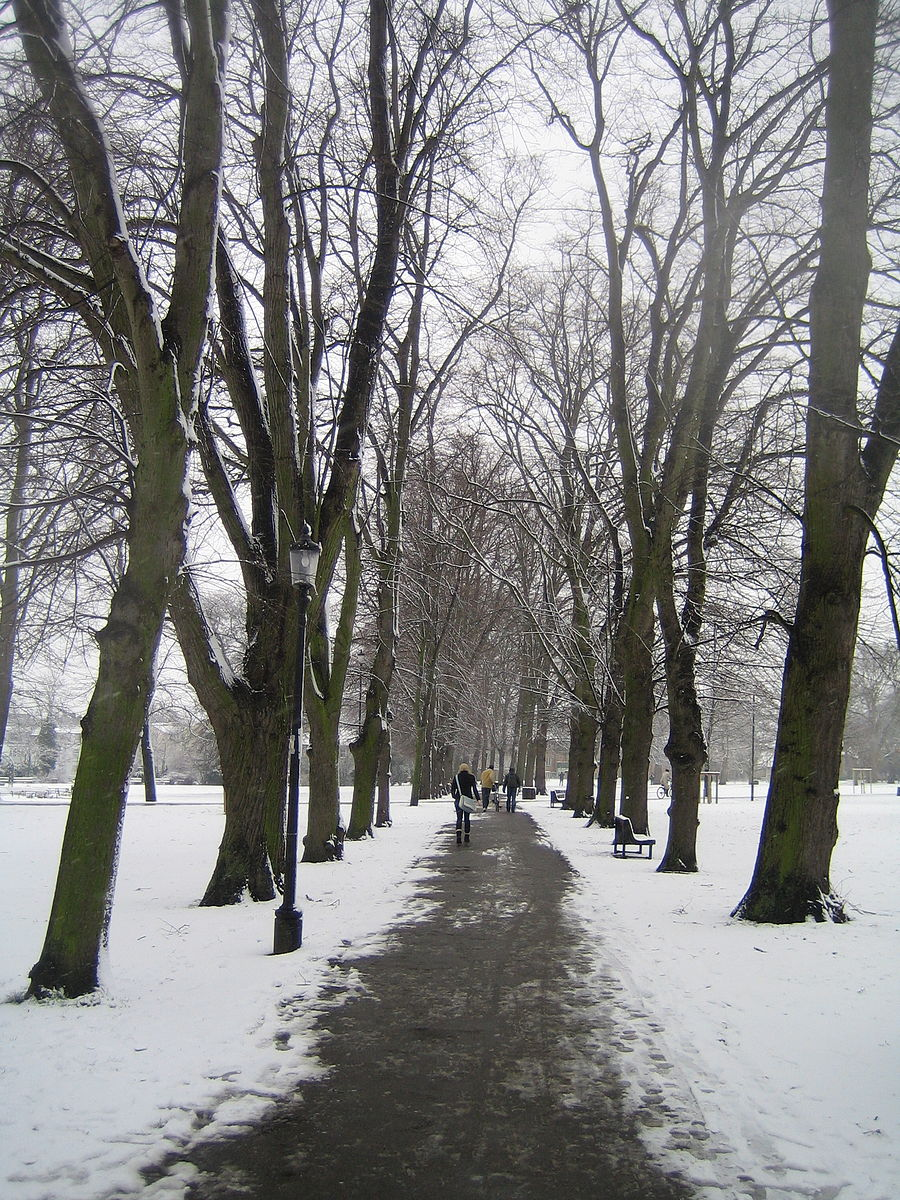
\includegraphics[width=\textwidth,trim=0 325 0 500, clip=true]{ChristsPieces}
\end{center}
\vspace{-.4cm}
\captionsetup{font=footnotesize,width=.47\textwidth}
\caption{\textsl{Park}: Christ's Pieces, Cambridge, UK.
% Public domain.
\label{christs-pieces}}
\end{figure}
%\vspace{-1.1cm}
%\end{wrapfigure}

\subsubsection*{Example 2} 
Just as a university campus grows and changes over time, future
peeragogues will be drawn to new problems and patterns. They
will trace new paths and build new emergent structures (Figure
\ref{christs-pieces}).

\smallskip

\begin{framed}
\noindent 
\emph{What's Next in the Peeragogy Project}
\definecollection{ScrapbookWN}
\begin{collectinmacro}{\ScrapbookWN}{}{}
After pruning back our pattern catalog, we want it to grow again: new patterns are needed.
One strategy would be to turn the whole \emph{Peeragogy Handbook} into design patterns.
\end{collectinmacro}
\ScrapbookWN
\end{framed}


%\newpage
           % \label{sec:Scrapbook}
\section{Emergent Roadmap} \label{sec:Distributed_Roadmap}

Table \ref{tab:WhatsNextSummary} reprises the ``What's Next'' steps from all of the previous
patterns, offering another view on the Peeragogy project's
\patternname{Roadmap} in a concrete emergent form.

Architectual maverick Christopher Alexander asked the following questions to an audience of computer programmers \cite{alexander1999origins}: 
\begin{quote}
``What is the Chartres of programming? What task is at a high enough level to inspire people writing programs, to reach for the stars?''
\end{quote}
In order for humanity to pull itself up by its bootstraps, on this planet or any other, we need to continue to learn and adapt.

People who learn actively together talk to each other about material problems, share practical solutions, and constructively critique works-in-progress.  There are many different ways to go about this -- bug reports, mailing lists, writers workshops, Q\&A forums, watercoolers and skateparks are all places where peeragogy can happen.  In the Peeragogy project have found that the necessary ``reflection'' aspects of the process are particularly well-matched to Christopher Alexander's idea of a \emph{pattern language}, in which commonly occurring,  interconnected, elements of an optative design are refined until they can be described in terms of a simple template.  Indeed, thought of as a design pattern, 

Peeragogy typically takes place in mostly-horizontal relationships between people who have different but compatible objectives.  The techniques we describe with these patterns are in many cases ancient; one can compare, for instance, the Quechua communal working practice of \emph{mink'a}.  The underlying practices can be pursued with or without high technology and with or without the technique of design patterns.

The Peeragogy project is one of ``tens of thousands of projects in the traditions of world improvement \'elan -- without any central committee that would have to, or even could, tell the active what their next operations should be'' \cite[p. 402]{sloterdijk2013change}.  When we talk about ``next steps,'' we aim to clarify our own commitments, and show what can be realistically expected from us.  

Unless the project's plan is easy for people to see and to update,
they are not likely to use it, and are less likely to get involved.
The key point of the roadmap is to help support involvement by those
who \emph{are} involved.  The level of detail in the roadmap (and the
existence of a roadmap at all) should correspond to the felt need for
sharing information and to the tolerance of uncertainty among
participants.

\begin{table}
{\footnotesize
\begin{tabular}{|p{\textwidth}|}
\hline
\rowcolor{Gray!30} \multicolumn{1}{|l|}{\color{Black} \ref{sec:Peeragogy}. \patternname{Peeragogy}}\\
\hline
\vspace{-.5em}
\PeeragogyWN\\
\hline 
%%%%%%%%%%%%%%%%%%%%
\rowcolor{Gray!30} \multicolumn{1}{|l|}{\color{Black} \ref{sec:Roadmap}. \patternname{Roadmap}}\\
\hline
\vspace{-.5em}
\RoadmapWN
\\[.1cm]
\hline
%%%%%%%%%%%%%%%%%%%%
\rowcolor{Gray!30} \multicolumn{1}{|l|}{\color{Black} \ref{sec:Reduce, reuse, recycle}. \patternname{Reduce, reuse, recycle}}\\
\hline
\vspace{-.5em}
\ReduceWN
\\[.1cm]
\hline
%%%%%%%%%%%%%%%%%%%%
\rowcolor{Gray!30} \multicolumn{1}{|l|}{\color{Black} \ref{sec:Carrying capacity}. \patternname{Carrying capacity}}\\
\hline
\vspace{-.5em}
\CarryingWN
\\[.1cm]
\hline
%%%%%%%%%%%%%%%%%%%%
\rowcolor{Gray!30} \multicolumn{1}{|l|}{\color{Black} \ref{sec:A specific project}. \patternname{A specific project}}\\
\hline
\vspace{-.5em}
\SpecificWN
\\[.1cm]
\hline
%%%%%%%%%%%%%%%%%%%%
\rowcolor{Gray!30} \multicolumn{1}{|l|}{\color{Black} \ref{sec:Wrapper}. \patternname{Wrapper}}\\
\hline
\vspace{-.5em}
\WrapperWN
\\[.1cm]
\hline
%%%%%%%%%%%%%%%%%%%%
\rowcolor{Gray!30} \multicolumn{1}{|l|}{\color{Black} \ref{sec:Heartbeat}. \patternname{Heartbeat}}\\
\hline
\vspace{-.5em}
\HeartbeatWN
\\[.1cm]
\hline
%%%%%%%%%%%%%%%%%%%%
\rowcolor{Gray!30} \multicolumn{1}{|l|}{\color{Black} \ref{sec:Newcomer}. \patternname{Newcomer}}\\
\hline
\vspace{-.5em}
\NewcomerWN
\\[.1cm]
\hline
%%%%%%%%%%%%%%%%%%%%
\rowcolor{Gray!30} \multicolumn{1}{|l|}{\color{Black} \ref{sec:Scrapbook}. \patternname{Scrapbook}}\\
\hline
\vspace{-.5em}
\ScrapbookWN
\\[.1cm]
\hline

\end{tabular}
}
\caption{What's next for the Peeragogy project\label{tab:WhatsNextSummary}}
\end{table}

%% \subsubsection*{\hyperref[sec:Peeragogy]{Peeragogy}} 
%% \PeeragogyWN

%% \subsubsection*{\hyperref[sec:Roadmap]{Roadmap}} 
%% \RoadmapWN

%% \subsubsection*{\hyperref[sec:Reduce, reuse, recycle]{Reduce, reuse, recycle}}
%% \ReduceWN

%% \subsubsection*{\hyperref[sec:Carrying capacity]{Carrying capacity}} 
%% \CarryingWN

%% \subsubsection*{\hyperref[sec:A specific project]{A specific project}}
%% \SpecificWN

%% \subsubsection*{\hyperref[sec:Wrapper]{Wrapper}}
%% \WrapperWN

%% \subsubsection*{\hyperref[sec:Heartbeat]{Heartbeat}}
%% \HeartbeatWN

%% \subsubsection*{\hyperref[sec:Newcomer]{Newcomer}}
%% \NewcomerWN

%% \subsubsection*{\hyperref[sec:Scrapbook]{Scrapbook}} 
%% \ScrapbookWN

\newpage
 % \label{sec:Distributed_Roadmap}
\section{Conclusion}\label{sec:Conclusion}

In this paper we have drawn on our shared experiences in the Peeragogy
project and our individual experiences in other collaborations, and
have taken whatever we can from the collected wisdom shared by expert
collaborators.  Our aim has been to outline a new approach to
education drawing on the principles of free/open/libre software and
``open culture.''  In order to do this, we have have attempted to
offer a clear discussion of these principles, rooted in an actionable,
hands-on way of thinking about things.

The potential societal benefits of a free/open/libre approach to
learning and education seem huge.  This approach has certainly served
us well over the course of our three-and-a-half year long
collaboration.  However, serious challenges remain.  We envision the
Peeragogy project as mutual aid society for other collaborative
projects.  And yet, many educators are not eager to collaborate, and
many enthusiastic collaborators are not particularly eager to educate.
Nevertheless, there are numerous inspiring examples of peeragogy (by
any other name) -- ranging from institutional forms like the co-op
format undergraduate training at Northeastern University and the
graduate-level entrepreneurship program at UC Berkeley, to more
informal collaborations in hacker-maker spaces and critique groups
around the world.
%, the NSF's Research Experiences for Undergraduates program

We hope that the current paper will be of use to those people who work
in and are interested in nurturing the overlap between ``libre'' and
``learning.''  If we have adopted a somewhat provocative stance toward
those working in and around this intersection, it is not because we
believe we have the right answer, but because we believe debate and
discussion are necessary for progress.




\bigskip

%% {\fontsize{10}{12}\selectfont\raggedright\uppercase{Acknowledgements}} \label{sec:Acknowledgements}\newline
%% \vspace{-.2cm}
%% \noindent

\subsection*{Acknowledgements}
David Kane was the paper's shepherd for PLoP'15, and provided detailed
comments and many suggestions that improved the draft.  Philip Bachman
was our on-site shepherd, and Mary Lynn Manns was our workshop
facilitator.  In addition to their help, the paper also benefited from
discussions with Doug Breitbart, the late George Brett, and Marian
Petre, among others.  We are grateful to Amanda Lyons and Fabrizio
Terzi for their contributed images.

Joseph Corneli was supported by the Future and Emerging Technologies
(FET) programme within the Seventh Framework Programme for Research of
the European Commission, under FET-Open Grant number 611553
(COINVENT).

%\newpage
\bibliographystyle{splncsnat}
\bibliography{peeragogy-bib}

\vspace{-3cm}


\end{document}
